\begin{figure}[h]
    \centering
    \begin{subfigure}{.5\textwidth}
      \centering
      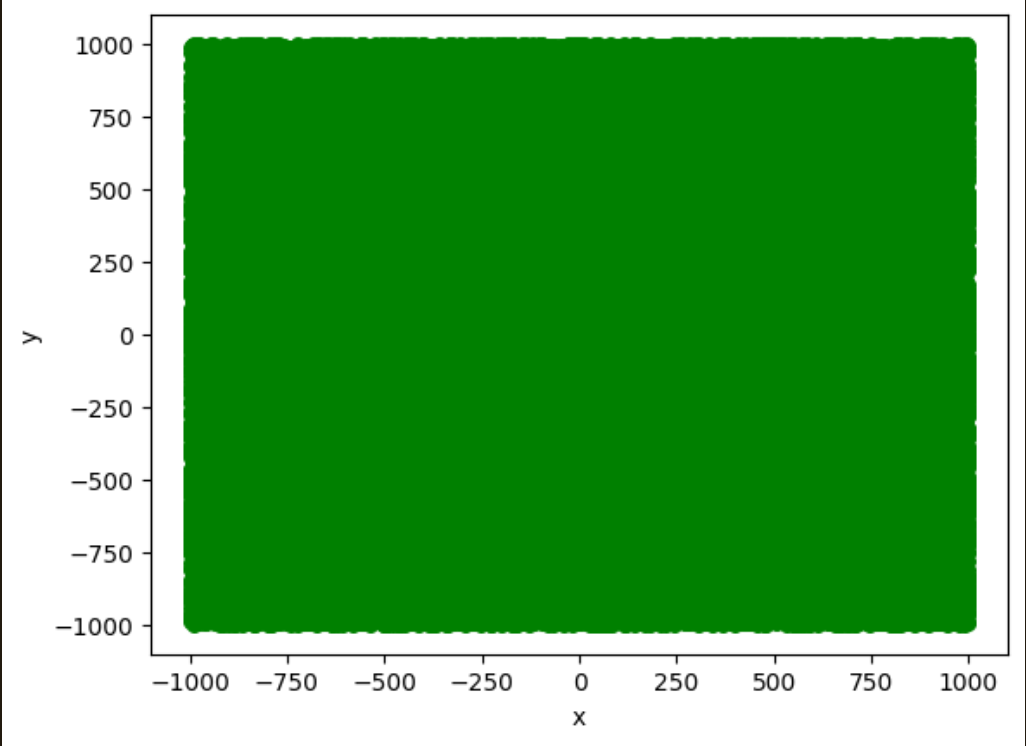
\includegraphics[width=.9\linewidth]{1.png}
      \caption{$10^5$ losowych punktów $(x, y) \in \left[-1000,1000\right]^{2}$.}
      \label{fig:sub1}
    \end{subfigure}%
    \begin{subfigure}{.5\textwidth}
      \centering
      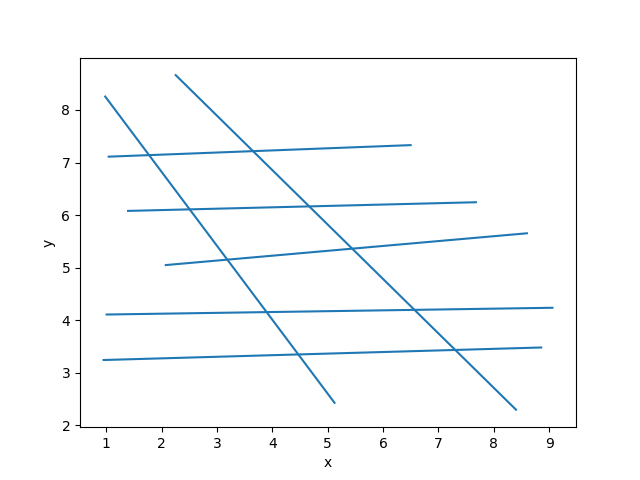
\includegraphics[width=.9\linewidth]{2.png}
      \caption{$10^5$ losowych punktów $(x, y) \in \left[-10^{14},10^{14}\right]^{2}$.}
      \label{fig:sub2}
    \end{subfigure}
    \label{fig:test}
    \end{figure}
    
    \begin{figure}[h]
    \centering
    \begin{minipage}{.5\textwidth}
      \centering
      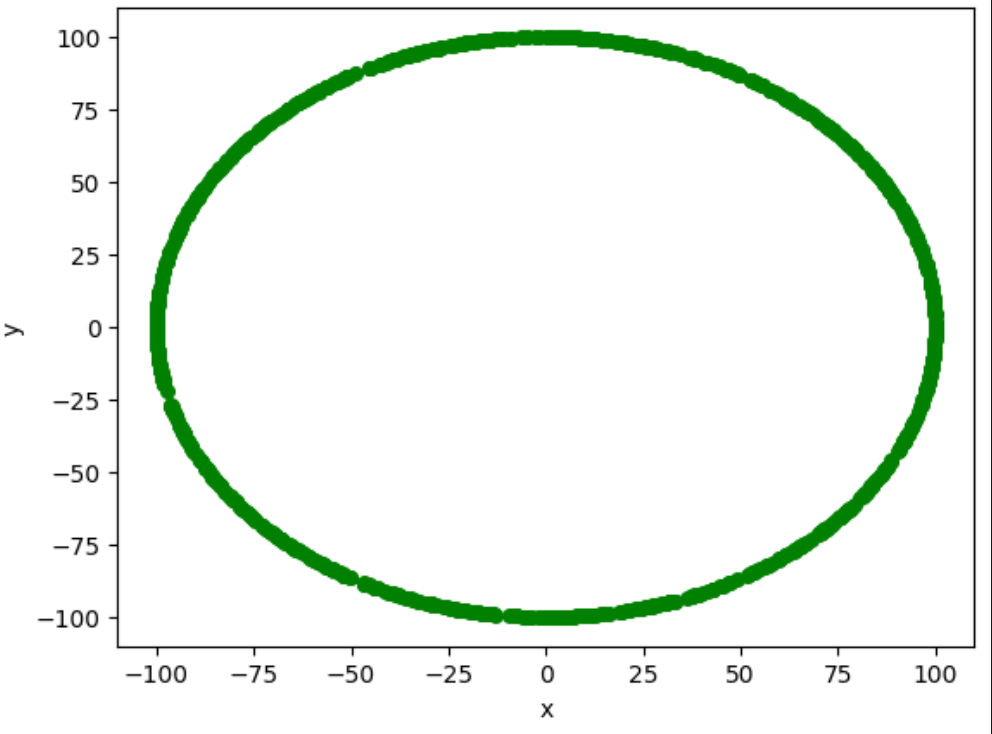
\includegraphics[width=.9\linewidth]{3.png}
      \caption{$1000$ losowych punktów leżących na okręgu.}
      \label{fig:test1}
    \end{minipage}%
    \begin{minipage}{.5\textwidth}
      \centering
      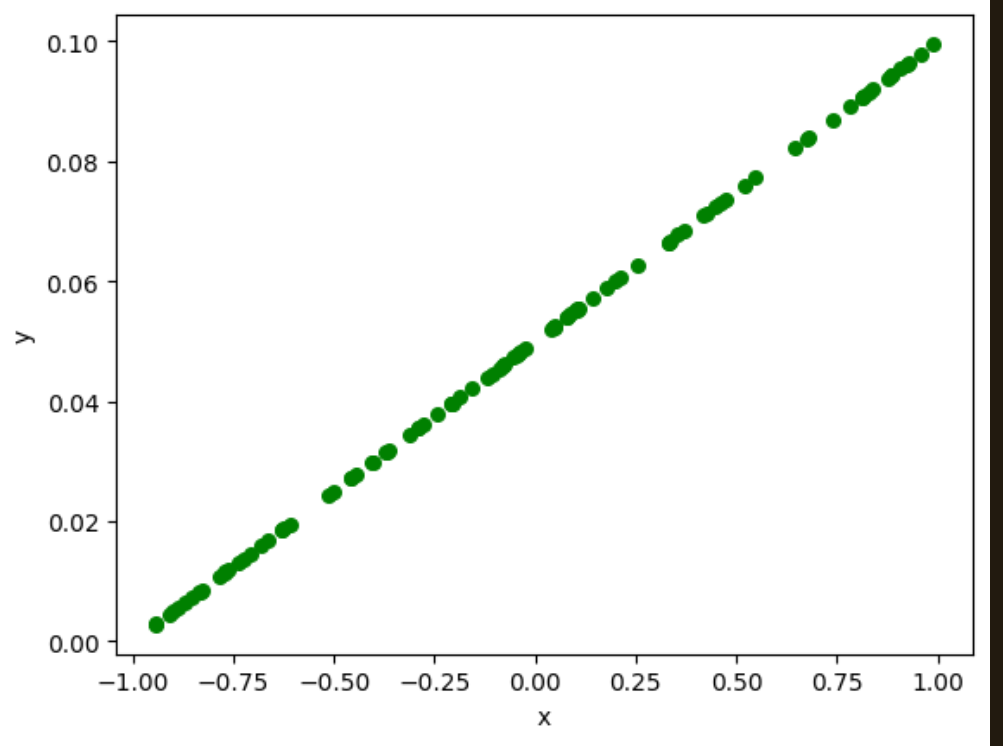
\includegraphics[width=.9\linewidth]{4.png}
      \captionof{figure}{$ 1000$ losowych punktów na prostej.}
      \label{fig:test2}
    \end{minipage}
    \end{figure}